% Chapter Template

\chapter{3D Models from Medical Imaging} % Main chapter title

\label{Chapter4} % Change X to a consecutive number; for referencing this chapter elsewhere, use \ref{ChapterX}
 
 %----------------------------------------------------


We present a use case, which shows how to derive a 3D model from a series of diagnostic images. The procedure here described is used to give an overview of the main functionalities of the software and the basic techniques of images and model management with the aim of providing a generic workflow, and some insights useful for the optimal resolution of specific cases. \\
The case presented here shows how to get a model of the mandible and how to prepare it for printing. The presented procedure is well suited to the extraction of models of organs with a strong contrast to surrounding tissue, such as bone tissue in CT.

\section{Image anonymization}
Before starting to work with images we must ensure that these do not contain sensitive data with which we can trace the patient's identity. In this case we will use the open-source software \emph{DICOM Confidential}, developed by the team \emph{Data Intensive Research of the University of Edinburgh} \parencite{Reference46} \parencite{Reference146}. The software allows you to load a folder containing the images, which are then processed according to the defined directives. \\
When the software is opened, the graphical user interface (GUI) appears. Here is possible to upload the folder containing the set to be anonymized. \\
The entries \emph{Policy URI} and \emph{Workflow file} have to be filled. These are the indications on the workflow to be performed and on the anonymisation operations to be executed on the images. The software provides standard templates to be used. These can be modified as required, and are located in the path \path | C: Userpath \ DICOM Confidential | (where \path |C: Userpath \ DICOM Confidential | is the folder where the software was installed). \\
The output path is \path | C: Userpath \ DICOM Confidential \ data \ ANONYMISED |. Using the standard configuration files, each anonymized set will be recognized by the DICOM reading software (3D Slicer in our case) as belonging to the single patient "ANONYMISED", to which all the anonymized studies will be added. To be taken into account during the organization of the system.

\begin{figure}[h]
	\centering
	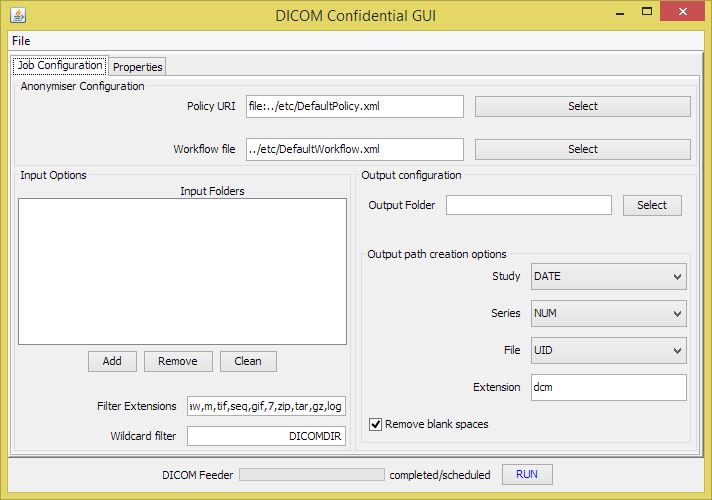
\includegraphics[width=0.9\textwidth, keepaspectratio]{gui_dicomConf}
    \caption{Schermata principale del software \emph{DICOM Confidential}}
    \label{fig:gui_dicomConf}
\end{figure}

\section{Anonymized Images}
Is possible to download anonymised datasets from \emph{The Cancer Imaging Archive} \parencite{Reference47}, a database maintained by the \emph{The National Cancer Institute} (NCI) and the \emph{University of Arkansas for Medical Sciences} (UAMS) to support multidisciplinary research, together with the \emph{Cancer Genome Atlas} dataset \parencite {Reference48} \parencite{Reference49}. \\
Several studies with various imaging techniques are available, which give the opportunity to deepen the analysis of various segments of the body and the oncological diseases that may occur.
To use the images, follow the simple procedures described on the website. Once the data is obtained, it can be loaded directly onto the visualization software.
                             
\section{Open the dataset}
The images obtained can then be uploaded to 3D Slicer for viewing and processing. We will use a set of images downloaded from \emph{The Cancer Imaging Archive} portal, located within the \path | TCGA - HNSC collection, Subject ID: TGCA-BA-6868, scan: Neck BW Axial|. \\
The software uses the \emph{DICOM} module \parencite{Reference50} to load and manage diagnostic image sets. The \emph{Volume Rendering} module can be used to display a rendered image. \\
With the \emph{Crop Volume} module it is possible to cut the volume part of our interest (Region of Interest, ROI), to lighten the computer from data that are not needed at the moment; it will be very useful later when we work with the models. In this example we want to create a model of the \emph{\textbf{mandibular bone}}, so we orientate the ROI in a way that contains the maxillary bones, and apply the modification.

\begin{figure}[h]
\centering
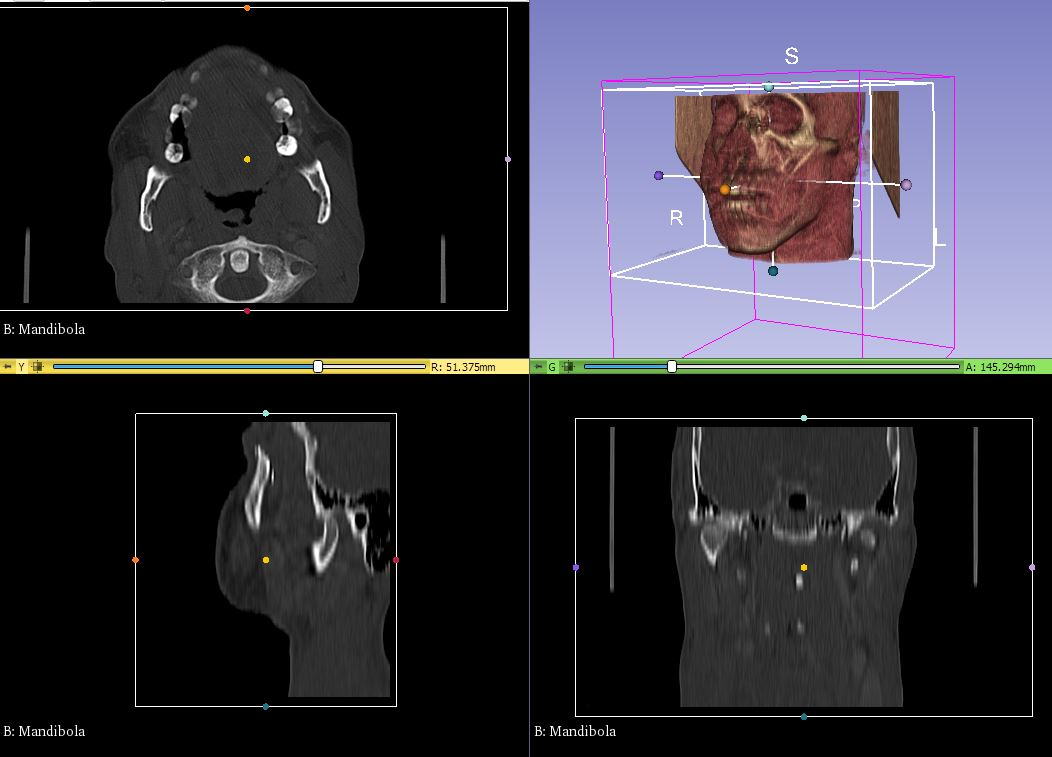
\includegraphics[width=0.8\textwidth, keepaspectratio]{crop1}
\caption{crop module used to select the upper and lower jaws region}
\label{fig:crop}
\end{figure}
\vspace{-10pt}

\section{Images segmentation and model creation}
We can then start the segmentation, using the \emph{Segment Editor} module. This module contains several tools that allow us to highlight the areas of the images of our interest. Since we want to extract the model of a bone, the mandible, a quick method is to use the \emph{bone density range} to quickly highlight the region of our interest. Then with the \emph{Add} button we add a segment and select the \emph{Threshold} tool which allows us to select a density range to highlight. The \emph{Data Probe} tool at the bottom left gives us information about the point in the image where the mouse tip is located, and contains an entry indicating the density at the point.
Selecting the threshold we look for a compromise between completeness in capturing details and cleaning in the segmentation mask. We have the possibility to perform a manual finishing of the segmentation, so we can leave some unselected area from the threshold to have a greater cleaning between the parts to be segmented. We consider that the selected areas must be separated to be treated as different segment, except if a different segment is used for each area; in that case the selection voxels can be adjacent without merging the volumes into a single object.\\
However, it is important to select the areas of interest in the best way, and in the CT we are segmenting a delicate point for the correct jaw separation is in the area of the condyles, where the selection is continuous with that of the anterior wall of the glenoid cavity of the temporal bone. Another point that have to be separated is the posterior region of the dental arch, at the level of the occlusal plane, where the teeth of the jaw are probably joined to the antagonists.

\begin{figure}[h]
\centering
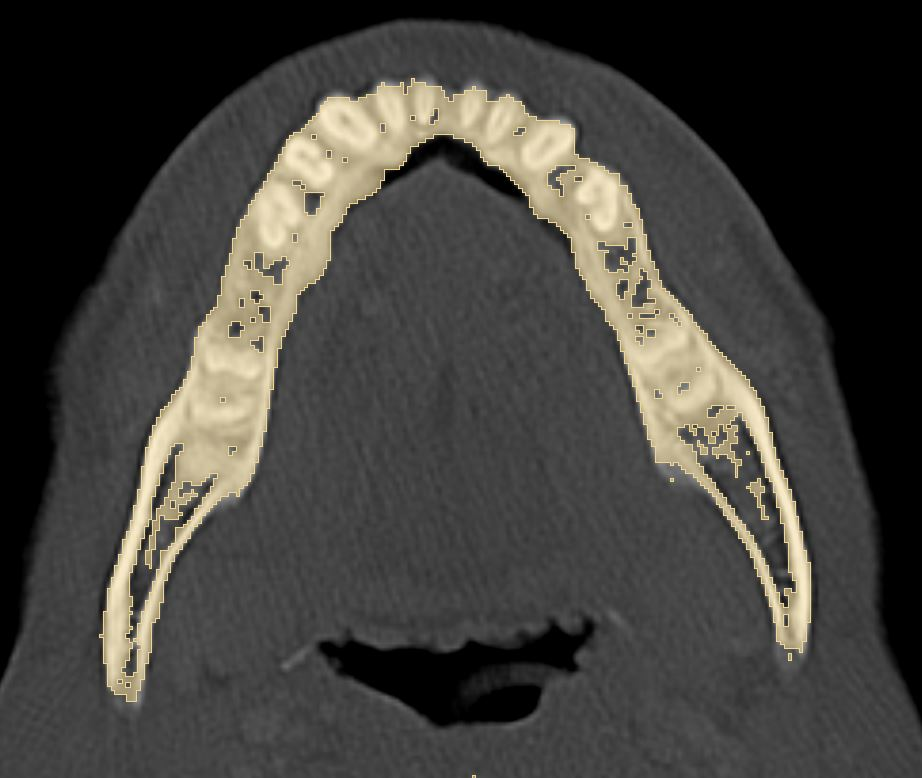
\includegraphics [width=0.6\textwidth, keepaspectratio]{origin_label}
\caption{Selection of mandibular bone and lower dental elements; \emph{threshold} 220 - 3071 HU; removal of small voxel groups: \emph{Island}> \emph{remove small island (minimum voxel=1000)}.}
\label{fig: origin_label}
\end{figure}

Once the threshold selection has been applied, we see that a mask has been created on the voxels that fall within the selected density range. This mask can be modified manually, adding any missing areas and separating the parts of our interest from the adjacent ones. By clicking on the button \emph{Show 3D} we can see the preview of the 3D model created by the segmentation; this option is useful to see if the selected areas correspond to the model we want to obtain, but when modifying the mask it is better to deactivate the option to save computational resources, and activate the 3D visualization only when necessary. \\
The removal of the contact areas between two selected region, in our case the mandibular condyle and temporal condyle, is performed in 3D Slicer to speed up the subsequent processing of the model. A model could have been created after the use of the threshold, but the separation of two models in software such as Blender is longer and more complex than the simple selection/deselection of voxels that can be performed in 3D Slicer.

\begin{figure}[h]
\centering
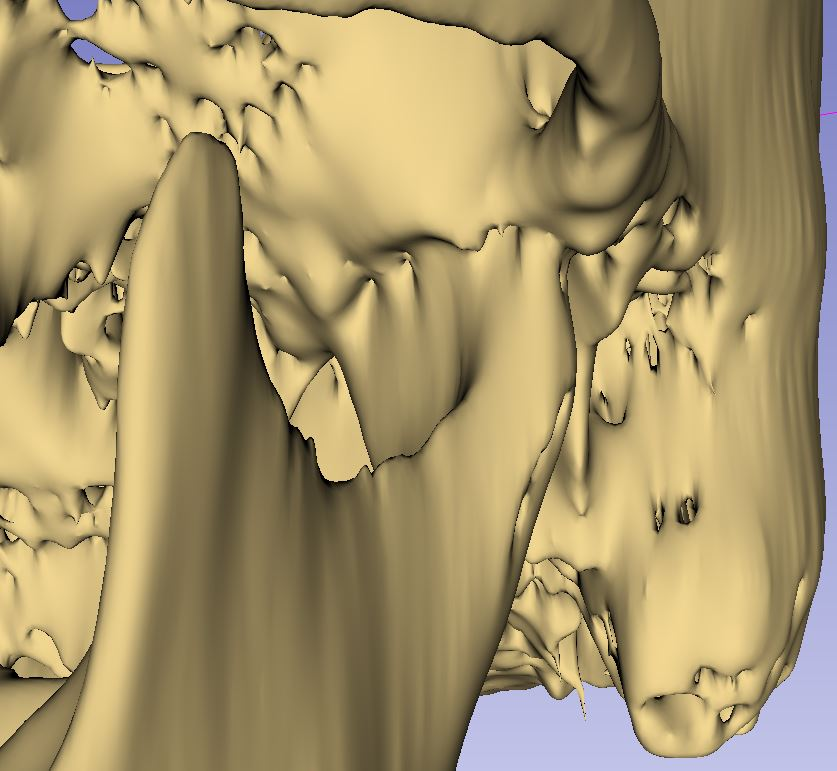
\includegraphics[width=0.4\textwidth, keepaspectratio]{fuso_condi}
\caption{3D reconstruction of the threshold segmentation of the mandible. The mandible is fused to the temporal bone.}
\label{fig:fuso_condi}
\end{figure}

We therefore aim to obtain from Slicer a 3D model as precise and clean as possible, to reduce the duration of subsequent steps, but also to create good quality segmentation datasets, which are useful for other purposes (data analysis, training set for Neural Network). \\
The \emph{Erase} tool allows to remove the voxels that do not need to be selected from the mask. \\
The \emph{Paint} tool allows the selection of voxels of interest that are not automatically selected by the threshold. \\
After finishing, we can use the \emph{Island} tool with the \emph{Keep Selected Island} option enabled; clicking on the jaw selection mask. If this island is separated from the rest of the selection we will have correctly performed the separation, which we can control by showing the model with the button \emph{Show 3D}. If we also want the model of the rest of the selection, we can click on the \emph{Undo} button to go back one step and retrieve the island containing the jaw and part of the skull.\\
We can create two separated segment: one for the mandible and one for the skull. We add a segment from the \emph{Add} button and we select it; using the \emph{Island} tool with the \emph{Add Selected Island} option we click on the skull mask and it will be added to the new segment. Separating objects into segments causes the spatial relationship between the parts to be lost, so if the parts need to be in a particular relation the \emph{Merge into single file} option must be selected to export the model as a single .stl file. It is then possible to separate this single model in its two components with the Blender software. \\
Then go to the module \emph{Segmentation}, where from the menu on the left we find the window \emph{Export to File}; select the destination folder and export the files in .stl format.

\vspace{-10pt}
\begin{figure}[h!]
\centering
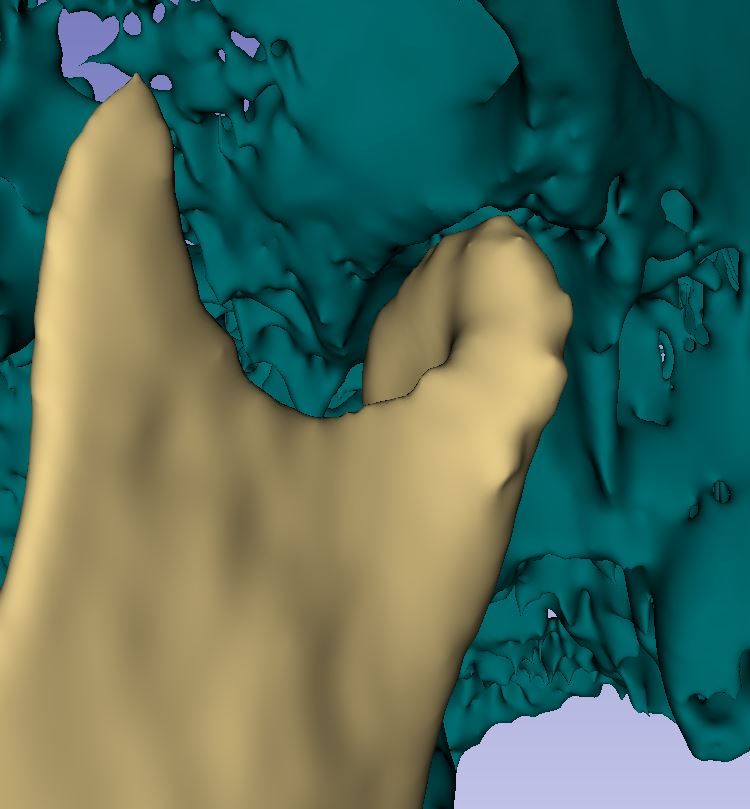
\includegraphics [width=0.4\textwidth, keepaspectratio]{sepa_condi}
\caption{Mandible separated from the temporal bone. The separation was done manually with the erase and paint tools. After separation a Segment for the jaw (yellow) and one for the skull (blue) were created.}
\label {fig: sepa_condi}
\end{figure}
\vspace{-15pt}

\newpage

\section{Model processing}
We import the model obtained in to MeshMixer and in the \emph{Analysis} menu we select the \emph{Inspector} tool. This function essentially has the task of detecting faults that must be resolved in order to have a closed model (\emph{manifold}) and to remove components separated from the main mesh. It is useful for preparing a model for 3D printing, where it is necessary that the model is precisely closed,  \emph{watertight}. This tool is useful for solving small problems with the mesh, but complex situations may require manual repair, which can be performed in this software as well as with Blender and MeshLab.

\begin{figure}[h]
\centering
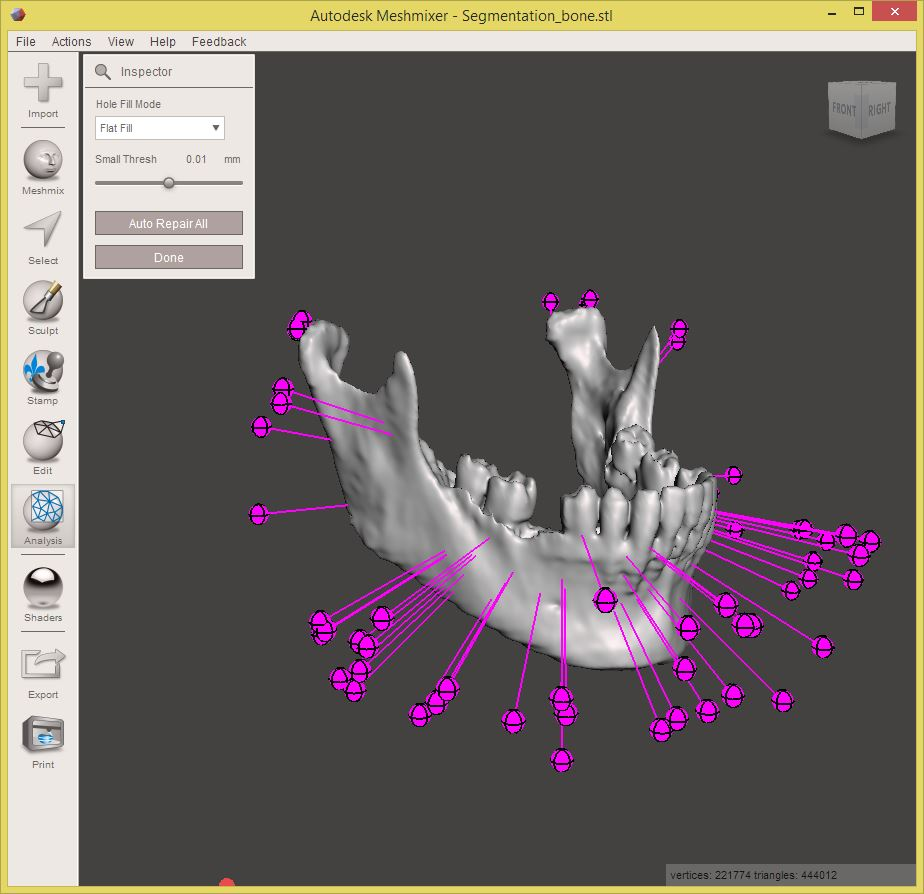
\includegraphics[width=0.8\textwidth, keepaspectratio]{inspector}
\caption{\emph{Inspector} tool in MeshMixer. Each violet indicator marks a fault in the mesh that can be fixed clicking on it.}
\label{fig:inspector}
\end{figure}

The model can then be exported to Blender to perform a smoothing. In Blender \emph{Modifiers} menu, select the \emph{Smooth} modifier. This is a function that smooths the surface of the object, causing a slight decrease in the object volume. In the instrument menu we can set the number of filter passages on the model; we find a compromise between smoothing and maintaining the original model dimensions. Another way to smooth the surface is to do it manually, with the sculpting tools \emph{sculpting} present in both Blender and MeshMixer. \\
After the model smoothing we inspect it to evaluate its quality; MeshLab can be used to compare two meshes. In our case we will measure the difference between the original model and the model obtained after 50 iterations of the \emph{smooth} modifier in Blender. When the models are aligned with each other, the procedure is to use the \emph{Hausdorff Distance} filter to evaluate the distance between the two meshes \parencite{Reference90}, \parencite{Reference91}. The software will return measurements related to the mesh sampling. \\

\begin{figure}[h]
\centering
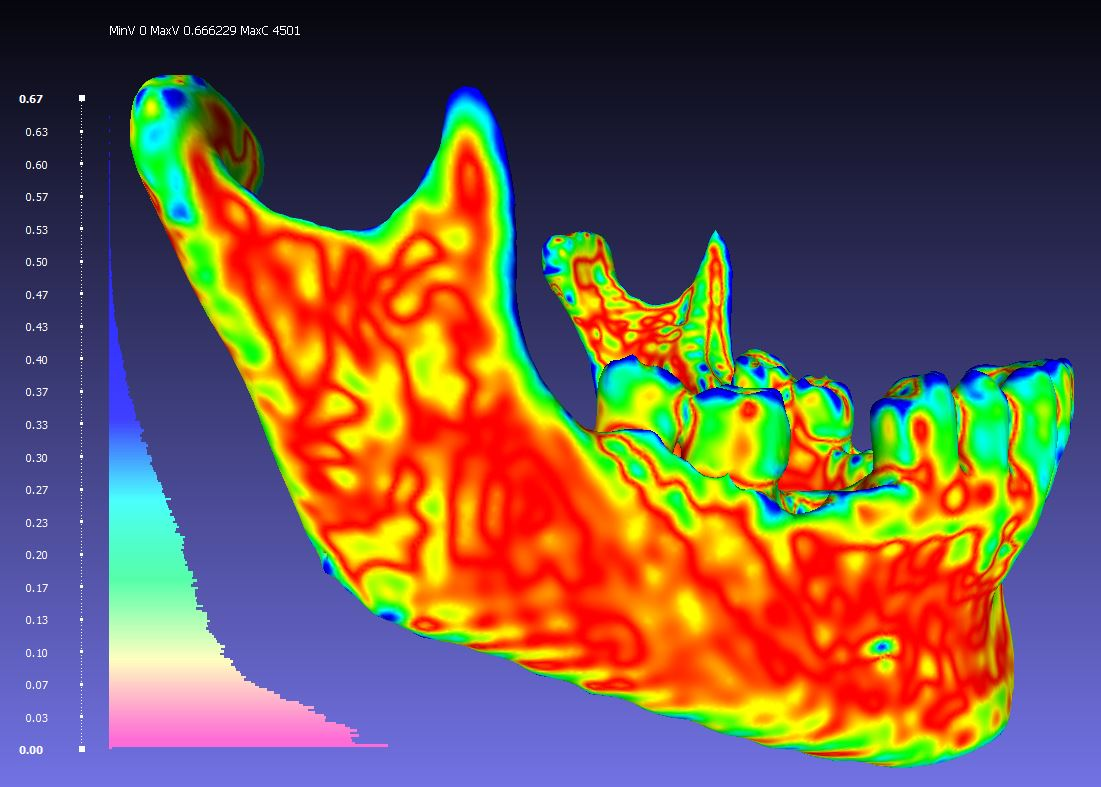
\includegraphics[width=0.8\textwidth, keepaspectratio]{hausdorff_smooth_clean}
\caption[LoF entry]{Hausdorff distance evaluation between the original model and the same model after 50 "Smooth" step in Blender. Legend goes from Red (no error) to Blue (max error).}

\begin{lstlisting}
Hausdorff Distance computed
Sampled 4657134 pts (rng: 0) on smooth_clean_Segmentation_bone.stl
searched closest on clean_Segmentation_bone.stl
min: 0.000000; max: 0.695190; mean: 0.116956; RMS: 0.154653

Values w.r.t. BBox Diag (181.472809)
min: 0.000000; max: 0.003831; mean: 0.000644; RMS: 0.000852 
Applied filter Hausdorff Distance in 29689 msec

Quality Range: 0.000000 0.666229; Used (0.006929 0.335713)
percentile (5.000000 95.000000) 
Applied filter Colorize by vertex Quality in 51 msec
\end{lstlisting}
\label{fig:hausdorff_smooth_clean}
\end{figure}

The mesh can then be colored to visually evaluate the discrepancy with the original mesh. To do this from the \emph{Filter} menu, select \emph{Color Creation and Processing} -> \emph{Colorize by Vertex Quality}. We can render the histogram from the menu \emph{Render} -> \emph{Show Quality Histogram}. \\
Keep in mind that the color scale goes from red to blue, where the \emph{red} indicates maximum correspondence with the original mesh, while the \emph{blue} indicates greater distance from the original mesh. The value is shown in model units, in this case millimeters. \\
As an alternative to MeshMixer it is possible to use MeshLab to perform more advanced mesh operations.
To remove regions separated from the main mesh, use the \emph{Filter} -> \emph{Cleaning and Repairing} -> \emph{Remove Isolated Pieces} tool, setting the minimum number of faces at a fairly high level, based on the number of faces shown in the bottom tool-bar. \\
To obtain a \emph{2-manifold mesh} \parencite{Reference92}, \parencite{Reference93}, in practical terms a \emph{closed mesh}: from the menu \emph{Filter} -> \emph{Cleaning and Repairing } use the functions: \emph{Remove Duplicate Faces}, \emph{Remove Duplicate Vertex}, \emph{Remove Unreferenced Vertices}, \emph{Remove Faces From Non Manifold Mesh}, \emph{Remove t-vertices From Non Manifold Edges}. \\ These commands clean up the mesh; to rebuild the 2-manifold mesh we use the command \emph{Filter} -> \emph{Remeshing, Simplification and Reconstruction} -> \emph{Screened Poisson Surface Sampling} \parencite{Reference95}, \parencite{Reference96}. This clean, 2-manifold reconstruction can be used for further processing. By performing an assessment of the quality of the reconstruction, it is noted that the agreement with the original mesh is very high.

\begin{figure}[h]
\centering
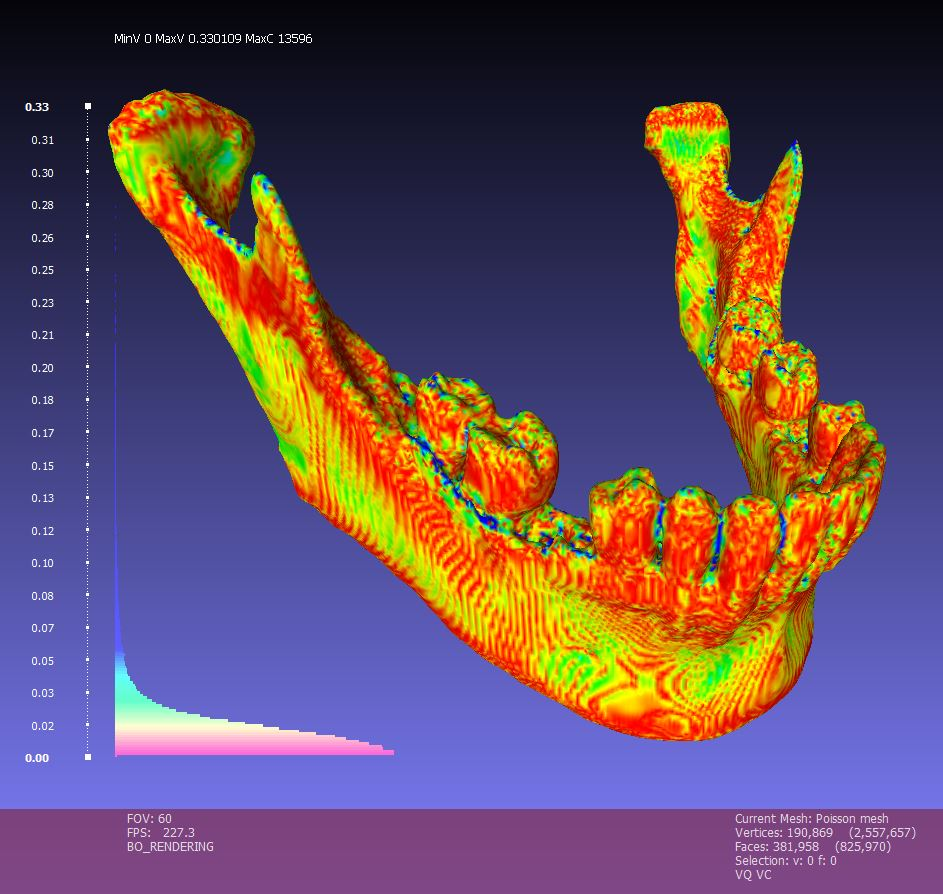
\includegraphics[width=0.75\textwidth, keepaspectratio]{noSeparate_poisson_clean_hausdorff}
\caption[LoF entry]{Hausdorff distance assessment after \emph{Screened Poisson Surface Sampling} algorithm.}

\begin{lstlisting}
Hausdorff Distance computed
Sampled 4195438 pts (rng: 0) on Poisson mesh searched 
closest on Segmentation_bone.stl
min : 0.000000 max 0.432402 mean : 0.019149 RMS : 0.031849

Values w.r.t. BBox Diag (182.226028)
min : 0.000000 max 0.002373 mean : 0.000105 RMS : 0.000175 
Applied filter Hausdorff Distance in 20254 msec
\end{lstlisting}
\label{fig:noSeparate_poisson_clean_hausdorff}
\end{figure}

We can make additional checks with the MeshMixer \emph{Inspector} tool to assess the need for further mesh refinements.
The model must then be exported in .stl format to prepare it for 3D printing.

\section{Slicing}
The digital model of the Jaw was obtained from the TC and processed to ensure a model suitable for printing. We will be slicing the model using the Cura software.\\
Load the model and select the \emph{Print Setup} > \emph{Custom} entry, to have the ability to fine-tune the printing parameters, which are initially hidden and must be activated. \\
The settings to be adjusted depend on several variables, including:

\begin{itemize}
\item the characteristics of the printer;
\item the characteristics of the model to be printed;
\item the printing material;
\item the accuracy and the mechanical properties expected from the object that we approach to print.
\end{itemize}

The environmental conditions in which you work are also to be taken into account, because for example some parameters may change between a print executed in a closed printer or in an open one.
The calibration of the printer and the knowledge of its specifications are fundamental for good printing result. Cura will generate printing instructions for the printer based on the printer specifications we entered in the \emph{Printers} > \emph{Machine Settings} menu. These settings are often updated with the addition of the most popular printer data, but for self-assembled printers the parameters must be entered manually. \\
With the calibrated printer and the information correctly entered in Cura, the model will be displayed in the software and will be sliced with the parameters entered. Once the slicing procedure has been completed we will be able to see the model layer by layer (\emph{Layer View}).
The so obtained \emph{\textbf{G-code}} can be used by the printer to produce the model.

\begin{figure}[t]
\centering
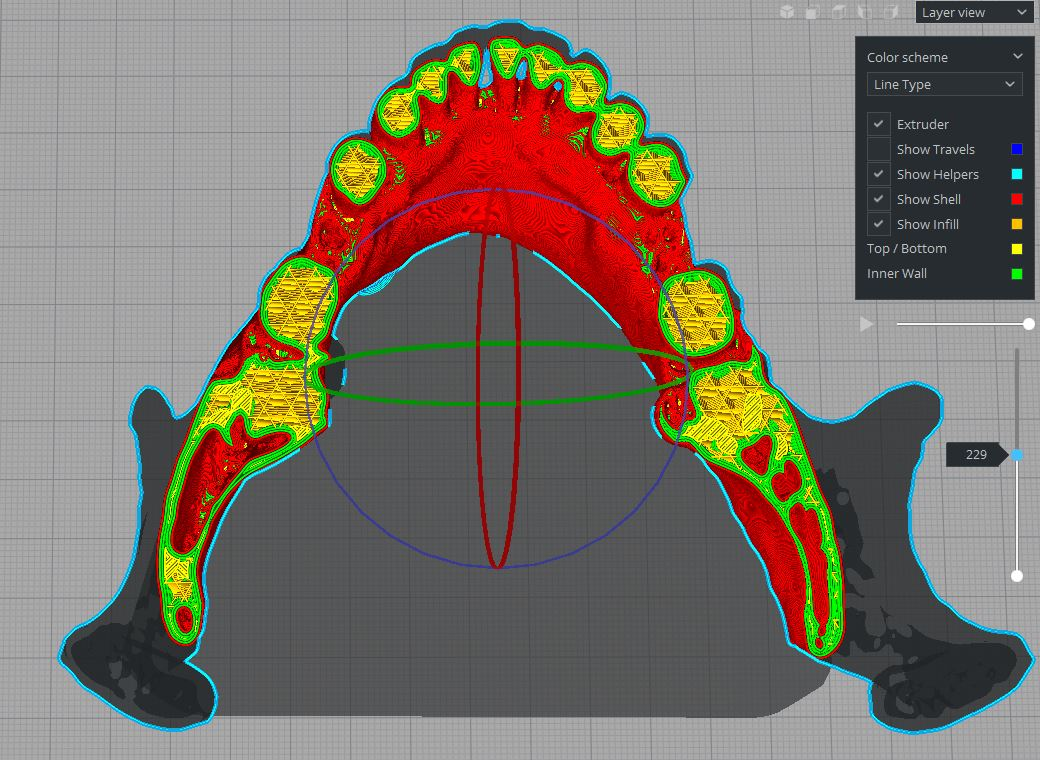
\includegraphics[width=\textwidth, keepaspectratio]{slicing}
\caption{Slicing of the mandible model in Cura.}
\label{fig:slicing}
\end{figure}

